
\documentclass[12pt, a4paper, twoside, openright]{book}

\usepackage{vuwthesis} % sets up some local things, mostly the front page

\usepackage{palatino} % sets palatino as the default font

\usepackage{url} % for typesetting urls



%\renewcommand{\baselinestretch}{1.00}


\begin{document}

\frontmatter
% Book style knows about front matter
% Report style doesn't so you need to set roman numbering etc yourself :-(

%%%%%%%%%%%%%%%%%%%%%%%%%%%%%%%%%%%%%%%%%%%%%%%%%%%%%%%

\title{Maintaining differently refactored views in Java}
\author{Paran Haslett}

\subject{Computer Science}
\abstract{
When developers collaborate on a project there are times when the code diverges. This could be due to refactoring or the code being reused in another project. It could even be due to throw away code or code used for debugging. This could at times also involve how the structure of the program is presented or the variable and method names that are being used. This is especially true if there is a piece of functionality that you wish to work on that differs from what everyone else is working on. In these cases you may need to refactor the code to best suit your changes before you apply them. The ability to have a separate view which although functionally equivalent to other views can present the code in a different form in these situations would be valuable. It enables the programmer to refactor or change the code with minimal impact on others. If the relationships between views are maintained it also could better recognise the changes that need to be communicated to other views or branches.
}
% Books don't normally have abstracts, and this is a bit of a hack

% Uncomment the appropriate degree
%\phd
\mscthesisonly
%\mscwithhonours
%\mscbothparts
% \otherdegree{DEGREE OR DIPLOMA NAME}



%%%%%%%%%%%%%%%%%%%%%%%%%%%%%%%%%%%%%%%%%%%%%%%%%%%%%%%




\maketitle


\chapter*{Acknowledgments}\label{C:ack} 

I would like to acknowledge the invaluable help of both my supervisors David Pearce and Lindsay Groves and also my wife Hye Eun Park who has been a great support during this thesis.


\tableofcontents


%%%%%%%%%%%%%%%%%%%%%%%%%%%%%%%%%%%%%%%%%%%%%%%%%%%%%%%

% book style knows about mainmatter
% if you are using report style you will have to rest page numbering etc.
\mainmatter

%%%%%%%%%%%%%%%%%%%%%%%%%%%%%%%%%%%%%%%%%%%%%%%%%%%%%%%

% individual chapters included here


\chapter{Introduction}\label{C:intro}

According to Bertino \cite{Bertino2012} \emph{Version control systems} provide a way of allowing multiple developers to collaborate. When multiple developers work on the same source code there is a risk that they have conflicting changes for the same portion of the source code.  One way of managing these conflicting changes is by ensuring only one person can edit a file at a time. This locking mechanism was recommended by Tichy \cite{Tichy1982} for the RCS version control system. Of course, the problem here is that one person can stop others from being able to edit the file. 

An alternative approach is to allow multiple changes to a file and to automatically resolve most of them in a process called a \emph{merge}.  The merge process compares the changes made in one version with the changes made on the other version. If the merge process determines that changes can coexist, it creates a merged file that contains all the changes. The changes that cannot be automatically merged are known as \emph{merge conflicts}.  The merge conflicts need to be manually checked and edited to form a merged file with the correct changes.

\begin{figure}[!t]
 \begin{center}
 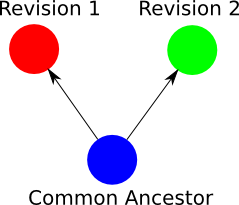
\includegraphics[scale=1]{introRevisions}
 \end{center}
 \caption{A file that has two different revisions}
 \label{fig:introRevisions}
\end{figure}



Internally the merge process needs to determine what changes have happened to both of the revisions being compared. In Figure  ~\ref{fig:introRevisions} there are two revisions that are derived from a common ancestor. It is possible to determine what has been deleted, inserted or changed by comparing each of the revisions against the common ancestor.  This is often done as a linear comparison of the source code for each revision. This works very well provided there has been no change in the order or structure of the file. However, if there has been a change where a block of source code has been moved from one place to another a linear comparison instead determines that two changes have occurred.  This is equivalent to deleting a block of source code from the common ancestor and inserting that source code elsewhere. It is possible that this change is not important to other programmers as the program behaves in the same manner even when source code is in a different order.  An example of this is if a Java programmer changes the order of methods within a program.  The program will behave in the same way as changing the order of methods does not change any functionality, however the source code is now different. The swapping of the order of the method is still counted as being two different changes even though the program behaves in the same manner as it did before the change took place.

Without any further analysis this change is recorded in the merged file even if the reordering was a personal preference for the programmer.  Although there has been no functional change the version control system will treat the relocation of blocks of source code exactly like a change in functionality.  Whenever a programmer attempts to update their code to incorporate any change in functionality, the change to the order of methods is also made to their code.  If a programmer is already familiar with the old structure of code and expects the code to remain relatively consistent the swapping of methods could be disconcerting.

Another issue that non-functional changes raise is an increase in the number of \emph{merge conflicts}. This could occur when two views have had a small amount of refactoring.  Since in both views the behaviour of the program has not changed it is possible that the merge conflict occurs about something trivial. An example of this could be different formatting or ordering methods alphabetically. For an ordinary text merge these changes to the structure of the source code require manual intervention. These issues highlight the need to develop smarter ways to merge.

It is becoming more important to have smarter merges because of the scale of many software projects and the number of developers working on them.
Large online repositories, like GitHub, contain many open source projects.
It is possible for these projects to make source code available to many developers at a time.
This means it is possible for two developers to work on the same project while having little personal contact.
Care needs to be taken when their individual work is combined.
Preferably most of the problems with merging their work should be automatically resolved however,
there still could be instances where either or both developers will have to figure out how the code should interact.
Having better automatic merges reduces the risk that time will be spent manually figuring out how different changes should be combined.

This thesis introduces the concept of maintaining multiple separate views which can be ordered differently but have functionally equivalent source code.
The purpose of these views is to reduce the number of changes introduced during a merge. 
It also explores a way of allowing a version control system to detect when there is a change in the source code but not a functional change in a program.
Examples of this are if items have been reordered, if comments have been inserted or there have been changes to the formatting. 
We developed the Refactor Categories Tool for the purpose of identifying these changes. 
We report on the design and implementation of this tool.
The Refactor Categories Tool is then used in an experiment evaluating a range of real-world benchmarks.


% We have used the Refactor Categories Tool we have created in an experiment 
% that iterates though all the revisions in the version source control for a 
% handful of Java projects.
% The Refactor Categories Tool detects
% 
% need to write about what we found here
 

\section{Overview}
In Chapter 2 we go over the background of version control, the longest common subsequence problem and refactoring as well as look at JDime, an existing tool for merging refactored views.
In Chapter 3 we discuss private views and what they could mean
In Chapter 4 we examine the Refactor Categories Tool, a precursor to developing private view. This will allow us to evaluate if additional merge operations are possible
In Chapter 5 we evaluate the results produced from the Refactor Categories Tool and determine what this could mean for our concept of private views.
In Chapter 6 we will conclude with some future work to make the concept of private view possible. 

% In this thesis we explore the idea of having private views that although 
% functionally equivalent can be refactored differently.
% A version control system allows us to have
% In this thesis we will examine the effects of non functional changes caused 
% by light weight refactoring of code on version control systems.
% To do this we will examine version control systems and how they allow 
% collaboration through merging.
% We will also examine refactoring and how it can change the code but retain 
% the same behaviour.
% We will some tools that could help when merging refactored code when it is 
% checked into an operating system.
% We especially focus on JDime to see if I can help us to build a private view 
% where external code changes are minimised.


\chapter{Different Views}
We want to have views that can have different but equivilent refactorings
This is so that people working on the same project can freely refactor with minimal interfarance to others

% find an example of a workplace situation where refactoring interfares with 
% others


\chapter{Using git}
Git provides the ability to seperate views but has difficulty merging them back together again.  

% provide an example
% 
% introduce gitless



\chapter{Different Views}
If the files have been greatly refactored then it becomes difficult to merge.  The traditional merge has been done using text comparison
% find an example


\chapter{Testing}
In order to test this we must first replicate the work of Apel and Le{\ss}nich

\section{Setting up the environment}
The work of Apel and Les{\ss}nich has mostly been done in Java.  There are a few exceptions including the linear programming libraries that need to be created.  As We are attempting to combine some of their work with Git it was decided to use JGit rather than the C implementation of Git. As the Java implementation may run a bit slower then in order to get a good timing test running we need to run redo the tests of JDime using JGit instead. 

Also the tests that Le{\ss}nich did on Jdime were from files rather than from a repository. It is necessary to set the files back up in the original repository structure to get a adequate baseline.

The tests I have written are based on simple changes and the range of refactoring available in the eclipse IDE.  They include such things as changing variable and method names 

Test name, expected optimal result, actual result
Changing comments, no change in target
Changing local variable names, no change in target, the method should be examined to ensure that all variables of that name are changed
Changing private variable names, no change in target,  the class should be examined to ensure that all variables of that name are also changed
Changing default variable names, no change in target, the  package should be examined to ensure all variables with this name are also changed. There is still a risk. A file that is in the same package that has not been placed in the appropriate source directory before the merge could no longer compile
% insert example
 
Changing protected variable names, target needs to conflict, The interface between this class and the inheriting class has changed.  The inheriting class could be from a different system.  A change in the variable name could mean that an external program does not compile or run.

Changing public variable names, target needs to conflict, The contract is also changing
Changing private method names, no change in target
Changing default method names, no change in target if the whole package is taken into account
Changing protected variable names, target needs to change as the inherited contract changes
Changing public variable names, target needs to change as contract is also changing 


\chapter{Conclusions and future work}\label{C:con}

In this thesis we presented the concept of maintaining private views in Java.
A private view presented here is an environment that allows a developer to import changes they want while avoiding hidden unwanted changes. 
This concept would also allow programmers to implement lightweight refactoring to their tastes, while minimising the impact on others.  
In evaluating what these private view will look like we used version control systems as a starting point.
There are some features of version control systems that already temporarily limit unwanted changes (e.g. branches).
However, during a merge any unwanted refactoring is imported. 
To this end we created the Refactor Categories Tool as a precursor to creating private views. 
This tool analyses the difference between two revisions such as encountered during a commit and identifies some examples of lightweight refactoring.
The way that the Refactor Categories Tool analyses these differences is by first parsing the source for both commits into a Java Abstract Syntax Tree (AST).
Once the AST is populated we then identify which parts of the AST match the differences we want to examine.
We then use the AST to identify additional features that have been changed. 
The features we have focused on are ones that do not change any functionality such as methods being moved or comments being changed. 
The results show that some of these lightweight refactorings are encountered in practice.
As the Refactor Categories Tool is a prototype it did not, unfortunately, select as many as we hoped.
We believe that it is possible to detect many more non-functional changes using more advanced identification algorithms.

\section{Future work}

In order to further the research into private views it would be useful to evaluate how the Refactor Categories Tool could be enhanced to detect more non functional changes. 
In addition to this some other tools could be adapted to create and evaluate the usefulness of private views.  
\subsection{Changes to the Refactor Categories Tool}

There are a number of ways that the Refactor Categories Tool could be changed to discover more moves, and renames:

\begin{itemize}

  \item At the moment the Refactor Categories Tool only examines moves that occur within a class, however, there could be non-functional changes that occur inside a method. 
An example would be if a local variable declaration was moved.
Sometimes this move would have no effect on the code and others it could cause the code to no longer compile.
  
  \item At the moment the refactor categories tool only compares matches within a limited scope (i.e. a class).  
  By allowing the Refactor Categories Tool to check other parts of the code, such as inner classes or even other files may also produce some interesting results.
Although we cannot guarantee that the moves discovered are valid ones this could give us more information about the source code we are examining.

  \item At the moment the Refactor Categories Tool only examines files that have been identified by JGit as being modified or renamed.
In some instances JGit could have incorrectly determined that a file as been deleted and reinserted rather than being renamed or moved.
This could happen easily since during a move or rename the a Java file changes the package reference and class name within a file.
This is especially true if the class has both been renamed and modified.

  \item Revising the scoring system for matching up inserts and deletes may produce some better results.
At the moment modifications are counted as two changes using the scoring system to match inserts and deletes.
Experimenting by reducing this value could improve the number of matches.

\end{itemize}




   

In addition to moves and renames, other lightweight refactoring may be of interest.
One of these are changes to access modifiers.
An example would be if a methods access changes from being private to being public.
Each of the method calls would then need to be rechecked to ensure that the change does not affect functionality.
Due to the possibilities of overloaded methods in Java this would be complicated.

An additional lightweight refactoring that could be considered is code that has been duplicated.
This could be done in a similar manner as how the Refactor Categories Tool check for code that has moved.
If we also check for code that has been modified slightly we may be able to determine that a copy and paste has been used to generate new code.
However, at the moment the Refactor Categories Tool only considers code that has been changed.
If we want to analyse where code has been copied we would need to check the entire source for copies as opposed to just the items that have changed.

Comments could be associated with the AST Node they relate to.  
With this change would be possible to tell if changing a comment should be reflected in other views when there is a source code change. 
This change is difficult as it is hard to tell which block of code the comment refers to.  
One way this could be done would be to associate single-line comments at the end of the line with the AST Node that appears directly before them and other comments with the AST node that appears directly after them.  
This however is only a rough approximation so it may be helpful to also be able to specify exceptions to these rules by using annotations that tie the comment to a block of code. Annotations could also be used to specify how important the comment is.
If the comment is marked as unimportant it would indicate that it still should not be considered a change even if it differs between revisions.

The Refactor Categories Tool could be re-purposed to allow it to be used as a merge tool rather than a comparison tool that we are currently using it for.  
This would bring us a step closer to being able to realise the vision of having better separated private views.  

Performance of Refactor Categories Tool could be further enhanced by only parsing nodes that contain the text change.
This however would require major changes to the parser or rewriting it. There would also be the complexity of figuring out how to only partially parse a source code.
The benefits of rewriting the parser would save memory in addition to speeding up the parsing of Java code into AST nodes.


\subsection{Other lines of enquiry}

There are other tools that could be modified to determine when a refactoring has taken place.

JDime has already been investigates as part of this thesis.
Although JDime cannot recognise changes to comments or white-space it could be re-purposed.
If it could be converted into a comparison tool rather than a merge tool then code that has been refactored differently could be compared without the result being normalised.

According to Pace \cite{Pace} \emph{DiffJ} is able to find the functional differences between two revisions of Java source code.
When computing the difference DiffJ ignores a range of lightweight refactorings such as moved methods, moved imports and the code being reformatted. 
As it ignores comments and white-space however, it will not be able to determine if there have been comment based changes that may be important. 



% 
% future work: by keeping track of equivalences there is no need to retest 
% using the AST
% 


%%%%%%%%%%%%%%%%%%%%%%%%%%%%%%%%%%%%%%%%%%%%%%%%%%%%%%%

% and of course book style knows about backmatter
% \backmatter caused problems with appendices :-(
% and of course report style doesn't
%%%%%%%%%%%%%%%%%%%%%%%%%%%%%%%%%%%%%%%%%%%%%%%%%%%%%%%


%\bibliographystyle{ieeetr}
\bibliographystyle{acm}
\bibliography{Thesis}


\end{document}
